\addcontentsline{toc}{section}{Subsystems}

%-------------------------------------------------------------------------------
% Subsystems / Client Requests
%-------------------------------------------------------------------------------
\subsection{Client Requests}\label{subsec:clientRequests}

\subsubsection{Class Diagram}
\paragraph{Release 1}

\indent
In release 1, the client had 3 actions that could make through the request classes.
They could make, delete or save reservations.
The requirements only required that the user was able to make and delete a reservation, and that it would persist throughout the system.
In order to make up for the fact that undo was not present in the system, saving the reservations was a separate command to allow for not saving changes that were not wanted.
This was also a pretty poor implementation of the command pattern, as the invoker was never used, and each command was instantiated and removed at use.

\begin{center}
    \makebox[\textwidth]{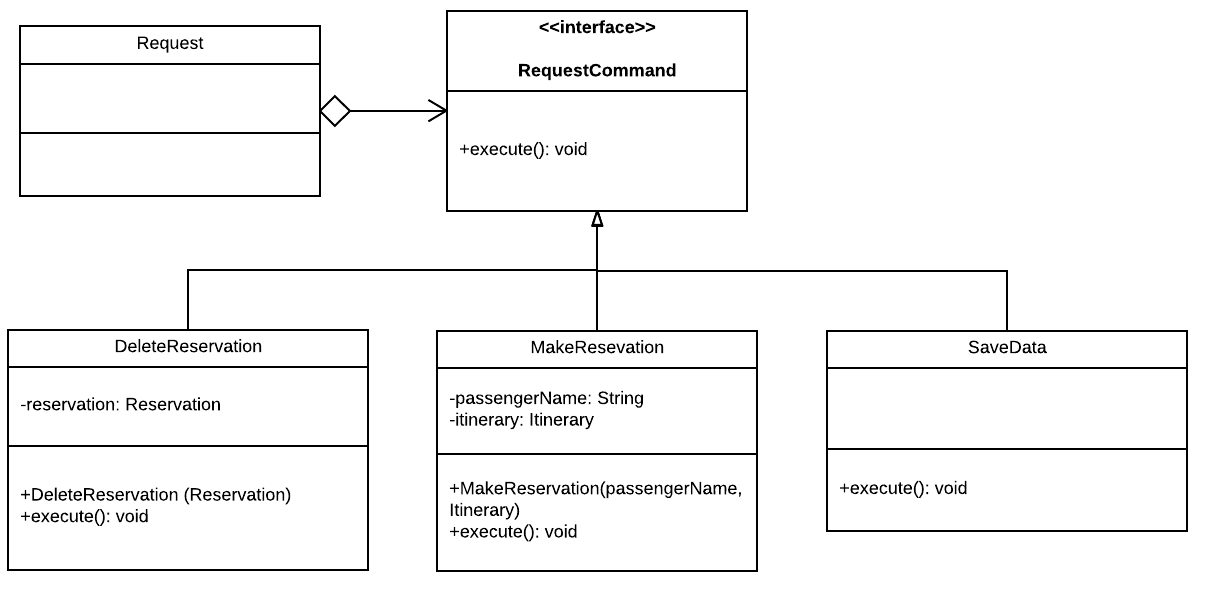
\includegraphics[width=\linewidth]{images/r1request.png}}
\end{center}

\paragraph{Release 2}

\indent
During release 2, the command pattern is moved around and used in a few places.
The requests from Release 1, are still in the client, and provide the undo/redo functionality as they are now meant to by the requirements.
However now they no longer interact with the datahandler directly, they now call routes in the server to perform commands.
Completely invisible to the user, or the client, the actions are then performed on the server.
Now as well as providing a command pattern, this section of the design also provides a proxy pattern for giving the client a place to hit, before all actions are done elsewhere.
A design choice made was to use the command and proxy patterns heavily modified here in order to make it work as we designed.

\subsubsection{Sequence Diagrams}

\paragraph{Release 1}

\begin{center}
    \makebox[\textwidth]{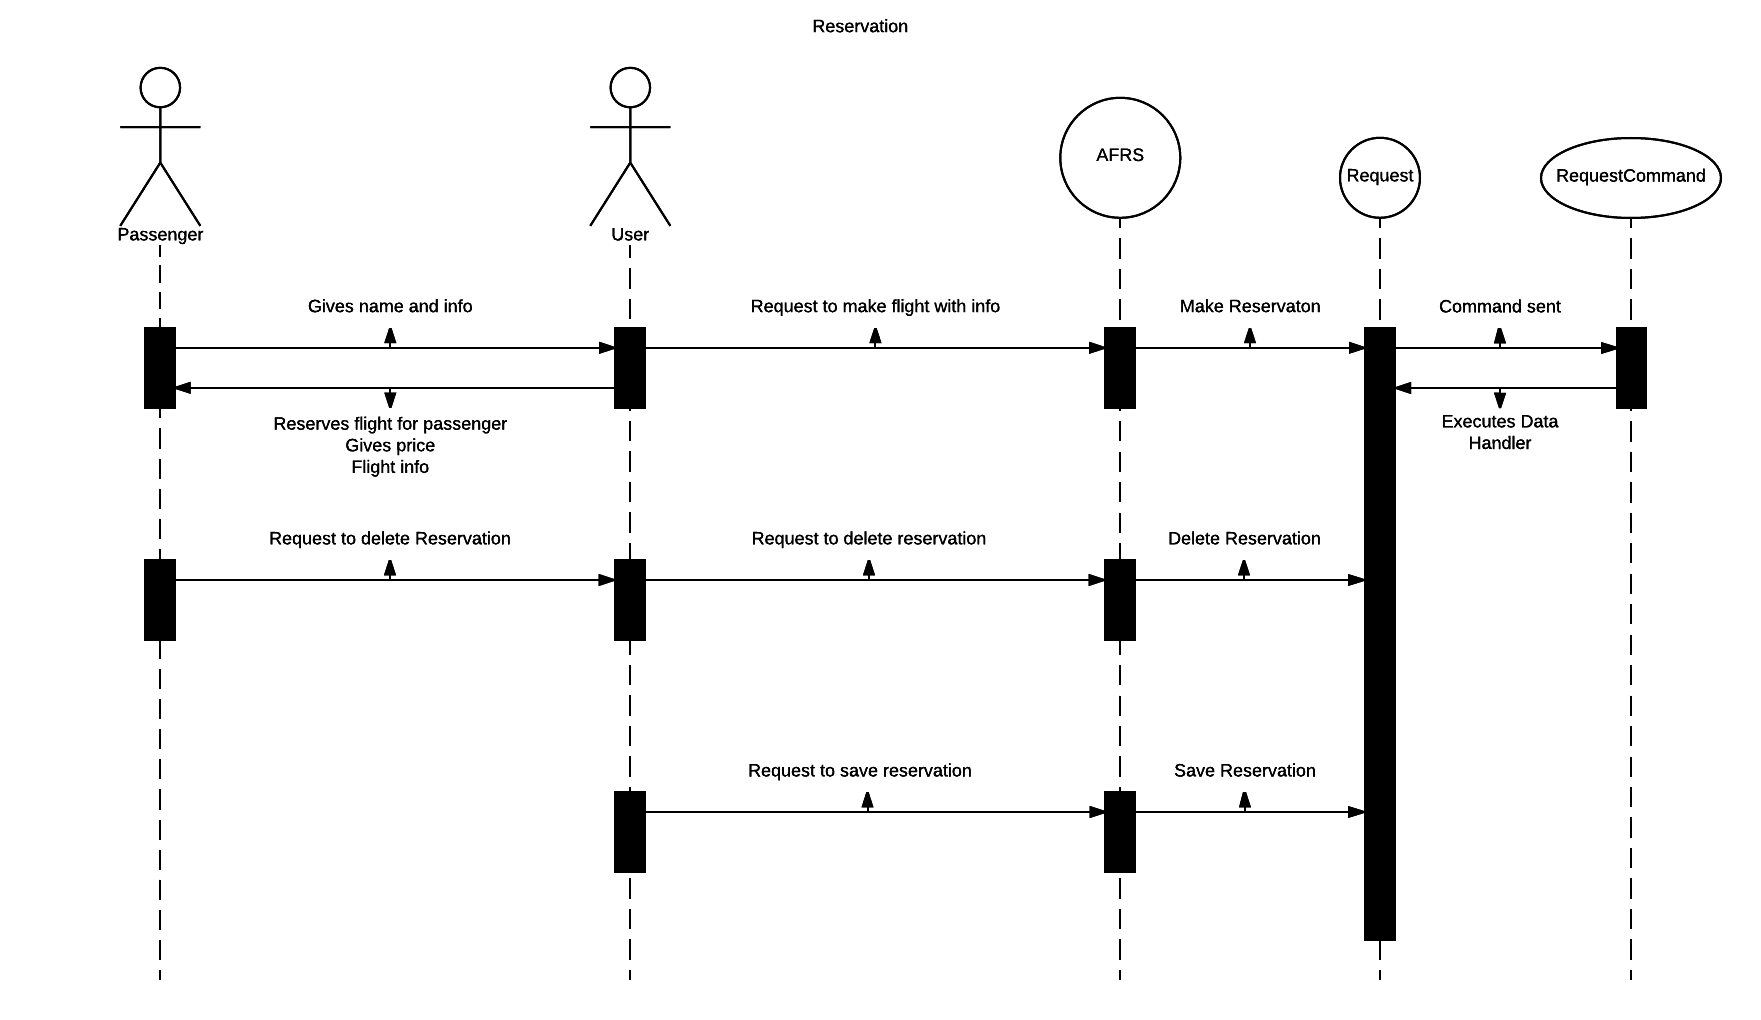
\includegraphics[width=\linewidth]{images/r1sequence1.png}}
\end{center}

\paragraph{Release 2}

\indent
In Release 2 we omitted the Invoker entirely as it was unnecessary. We also had to now account for undoing of commands. With this in mind, it was actually pretty easy to implement simple undo/redo functionality as long as we held a request object in memory to allow us to call the undo/execute commands.

\begin{center}
    \makebox[\textwidth]{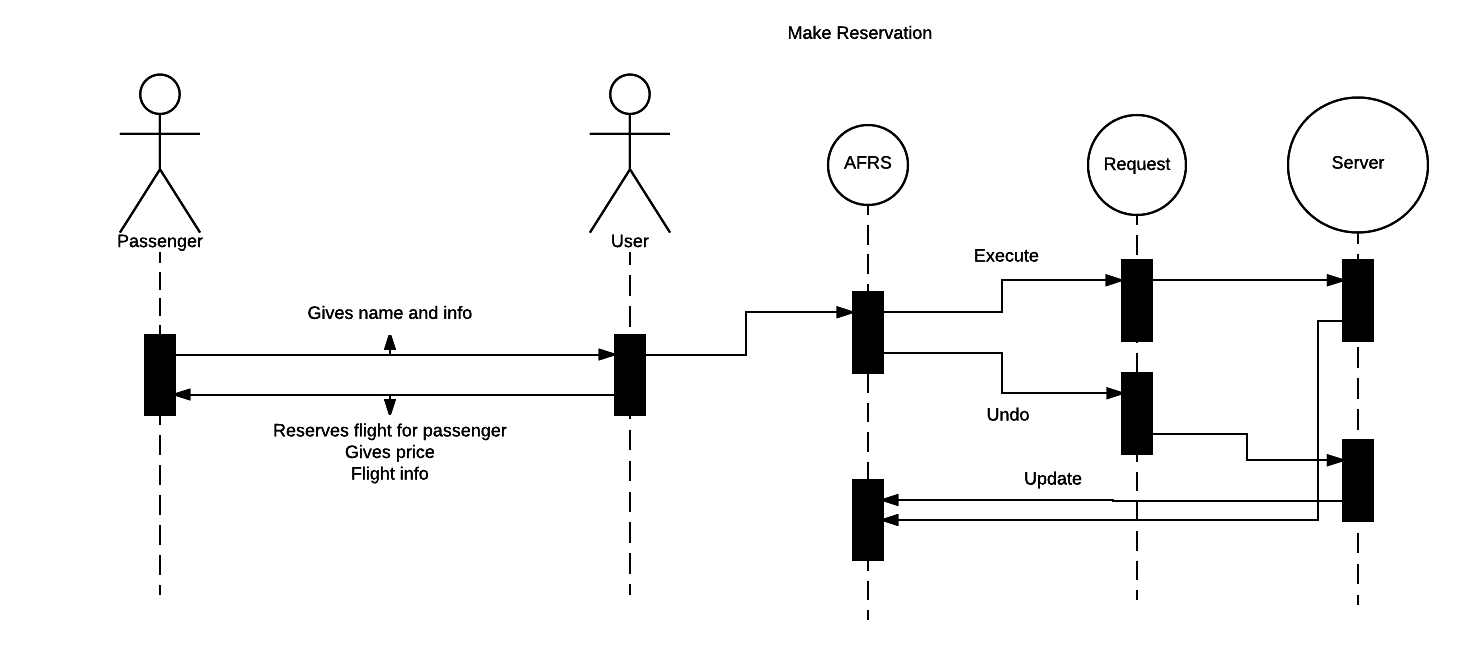
\includegraphics[width=\linewidth]{images/r2-makereservation-sequence.png}}
\end{center}

\subsubsection{GoF Card}
\begin{center}
    \begin{tabular}{ |p{4cm}|p{4cm}|p{7cm}|  }
        \hline
        \multicolumn{2}{|c|}{Name: Request} & \multicolumn{1}{|c|}{GoF pattern: Command} \\
        \hline
        \multicolumn{3}{|c|}{Participants} \\
        \hline
        Class & Role in GoF pattern & Participant's contribution in the context of the application \\
        \hline \hline
        RequestCommand & Command & The overall command which could be used to reuse an existing request as another one.
        Although not currently used in this fashion, it would be fairly easy to make the change. \\
        \hline
        MakeReservation & Concrete Command & Makes a new reservation object and adds it to the system.
        This does so without returning anything to the user, or informing the user about what commands are being performed. \\
        \hline
        DeleteReservation & Concrete Command & Deletes reservation object from the system.
        This does so by calling the class in the datahandler without exposing that to the invoker. \\
        \hline
        \hline
        \multicolumn{3}{|c|}{Deviations from the Pattern:} \\ \multicolumn{3}{|c|}{\parbox{0.9\textwidth}{
        \begin{itemize}
            \item No reflection/pointers involved for target method.
            \item Commands have more distinct methods.
            \item No Invoker class.
        \end{itemize} }} \\
        \hline
        \multicolumn{3}{|c|}{Requirements being covered:} \\ \multicolumn{3}{|c|}{\parbox{0.9\textwidth}{
        \begin{itemize}
            \item The AFRS shall track reservations.
            \item The system shall allow a client to make a reservation for an itinerary contained in the most recent query for flight information.
            \item The system shall allow a client to query for reservations for a passenger.
            \item The system shall allow a client to delete a reservation for a passenger.
        \end{itemize} }} \\
        \hline
    \end{tabular}
\end{center}

\newpage

%-------------------------------------------------------------------------------
% Subsystems / Itineraries
%-------------------------------------------------------------------------------
\subsection{Itineraries}\label{subsec:itineraries}

\subsubsection{Class Diagram}

\paragraph{Release 1 \& 2}

\indent
The design for Flights and Itineraries is one of the subsystems that is the most easily understood.
Flights and Itineraries share a common interface, and therefore can be used interchangeably by the rest of the system.
This use of the composite pattern is incredibly useful here, and because of that, no changes were made between R1 and R2.

\begin{center}
    \makebox[\textwidth]{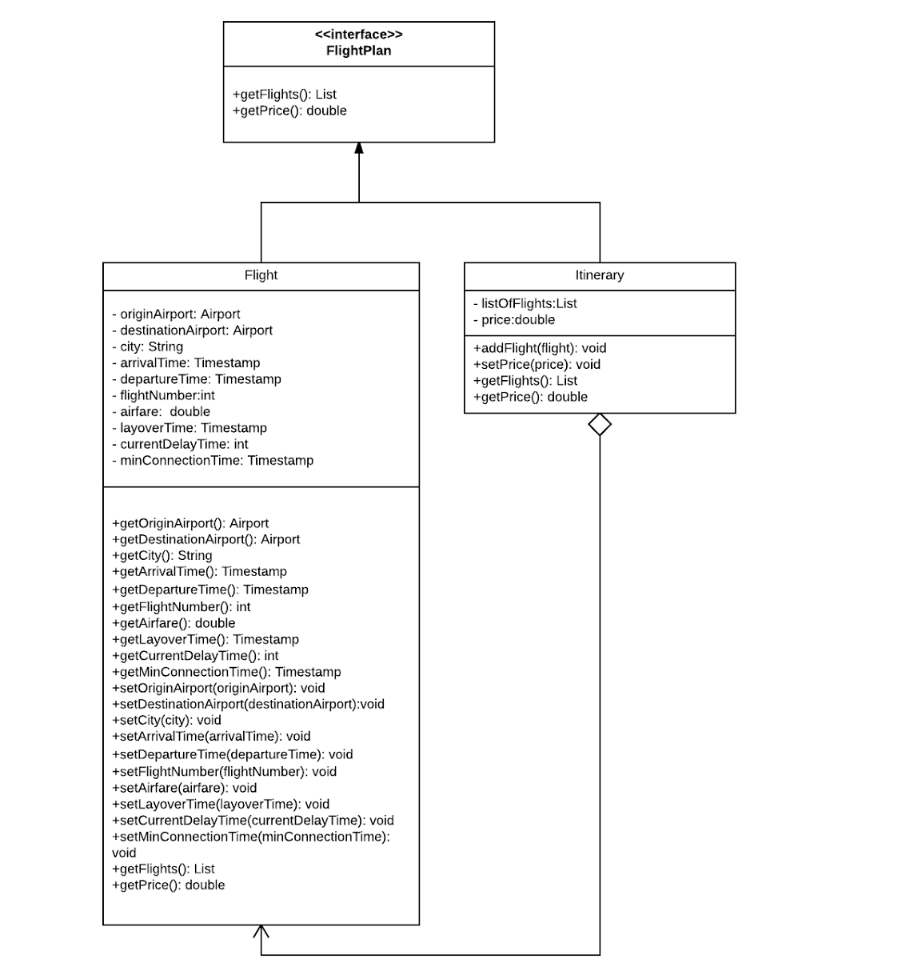
\includegraphics[width=\linewidth]{images/r1itineraries.png}}
\end{center}

\subsubsection{Sequence Diagrams}

\paragraph{Release 1 \& 2}

\indent
In Release 2, we added server route functionality to this subsystem in order to fit it in with the multi-concurrent user system.

\begin{center}
    \makebox[\textwidth]{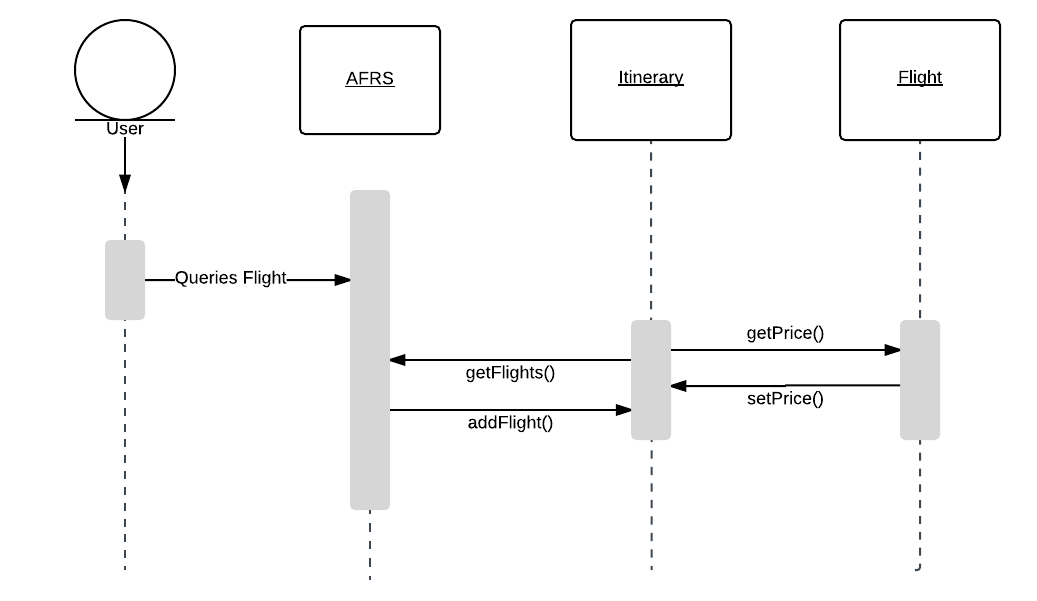
\includegraphics[width=\linewidth]{images/r1itinerarysequence.png}}
\end{center}

\newpage
\subsubsection{GoF Card}

\begin{center}
    \begin{tabular}{ |p{4cm}|p{4cm}|p{7cm}|  }
        \hline
        \multicolumn{2}{|c|}{Name: Itineraries} & \multicolumn{1}{|c|}{GoF pattern: Composite} \\
        \hline
        \multicolumn{3}{|c|}{Participants} \\
        \hline
        Class & Role in GoF pattern & Participant's contribution in the context of the application \\
        \hline \hline
        Flight Plan & Component & The component interface to uniform the leaf and composite. \\
        \hline
        Flight & Leaf & The actual flight object as it exists in the database.
        This will include all information needed to understand a flight. \\
        \hline
        Itinerary & Composite & The itinerary object, with a list of flights, and the total price for each of the flights inside of it.
        This itinerary is a possible set of flights to get from one destination to another. \\
        \hline
        \hline
        \multicolumn{3}{|c|}{Deviations from the Pattern:} \\ \multicolumn{3}{|c|}{\parbox{0.9\textwidth}{
        \begin{itemize}
            \item Leaf has many more encapsulated attributes than composite element.
            \item Composite does not contain Composites. It will only contain leafs.
        \end{itemize} }} \\
        \hline
        \multicolumn{3}{|c|}{Requirements being covered:} \\ \multicolumn{3}{|c|}{\parbox{0.9\textwidth}{
        \begin{itemize}
            \item The system shall store flight data for all flights between the cities in TTA's route network.
            Flight data shall consist of: origin airport, destination airport, departure time, arrival time, flight number, and airfare.
            An itinerary is a list of Flights that also stores the total airfare of each flight.
            This is used when a client creates a reservation with multiple legs.
        \end{itemize} }} \\
        \hline
    \end{tabular}
\end{center}

\newpage

%-------------------------------------------------------------------------------
% Subsystems / Sorting Algorithms
%-------------------------------------------------------------------------------
\subsection{Sorting Algorithms}

\subsubsection{Class Diagram}

\paragraph{Release 1 \& 2}

\indent
In Release 1, there were a series of classes whose sole purpose was to return a comparator.
During the discussion over the R1 design, it was determined that those extra classes were unnecessary to the use of the strategy pattern.
This was creating a series of classes that served no extra functionality, and simply abstracted a part of the system that never needed to be abstracted.

\begin{center}
    \makebox[\textwidth]{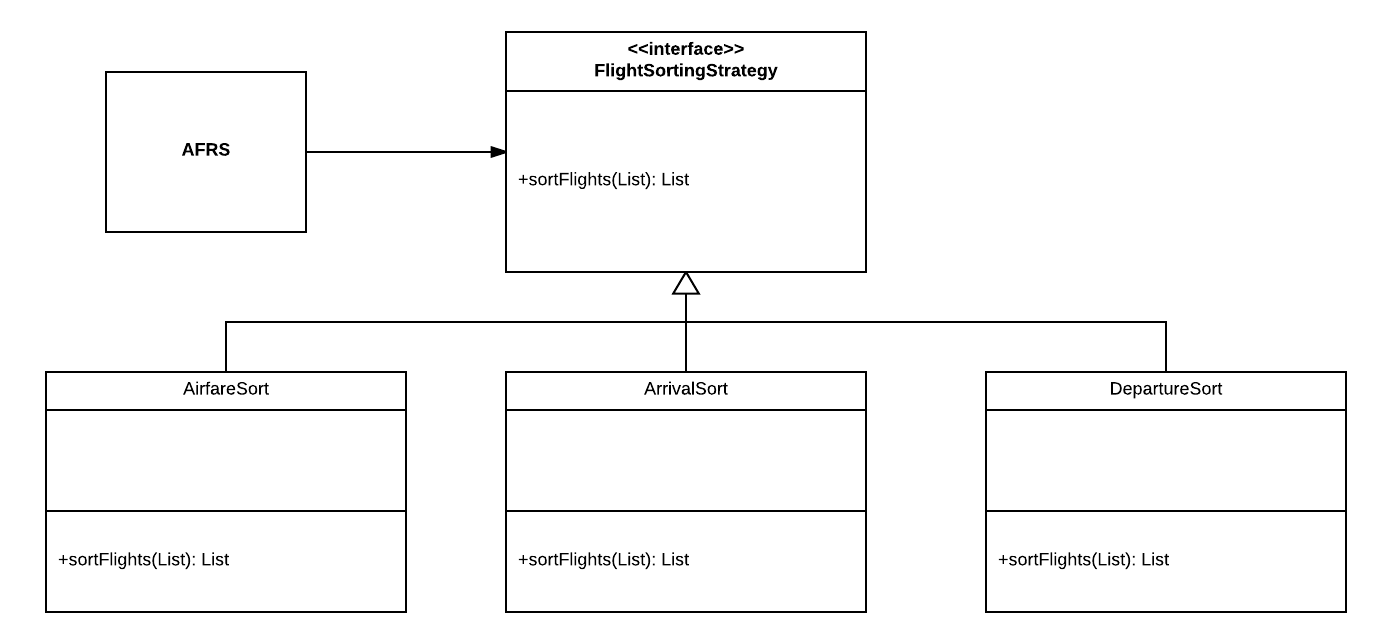
\includegraphics[width=\linewidth]{images/r1sortingclass.png}}
\end{center}

\newpage

\subsubsection{Sequence Diagrams}

\paragraph{Release 1 \& 2}

\begin{center}
    \makebox[\textwidth]{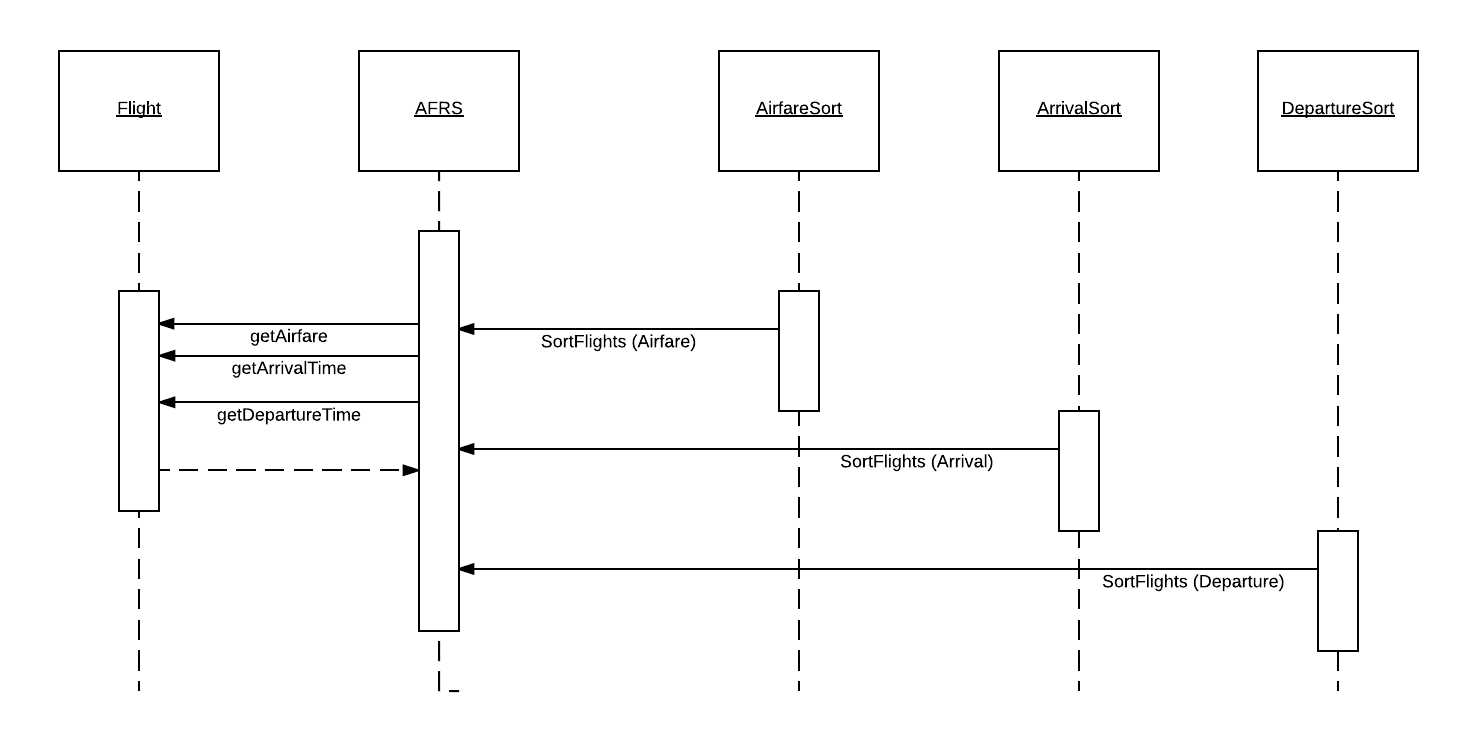
\includegraphics[width=\linewidth]{images/r1sortingstate.png}}
\end{center}

\newpage

\subsubsection{GoF Card}

\begin{center}
    \begin{tabular}{ |p{4cm}|p{4cm}|p{7cm}|  }
        \hline
        \multicolumn{2}{|c|}{Name: Sorting Algorithms} & \multicolumn{1}{|c|}{GoF pattern: Strategy} \\
        \hline
        \multicolumn{3}{|c|}{Participants} \\
        \hline
        Class & Role in GoF pattern & Participant's contribution in the context of the application \\
        \hline \hline

        AFRS & Context & Executes the strategy \\
        \hline
        FlightSortingStrategy & Strategy & An interface for multiple strategies for sorting flights \\
        \hline
        AirfareSort & ConcreteStrategyA & An algorithm for sorting airfare.
        It orders all flights and itineraries by using a Comparator implementation that compares price of two flights.
        Flights are ordered from least to most expensive. \\
        \hline
        ArrivalSort & ConcreteStrategyB & An algorithm for sorting arriving times.
        It orders FlightPlans by using a Comparator implementation that compares the Date objects of the last flight in the FlightPlan’s arrival time.  \\
        \hline
        DepartureSort & ConcreteStrategyC & An algorithm for sorting departing times.
        Using an implementation of the Comparator interface that compares two Date objects for the departure of the first flight in a FlightPlan.  \\
        \hline

        \hline
        \multicolumn{3}{|c|}{Deviations from the Pattern:} \\ \multicolumn{3}{|c|}{\parbox{0.9\textwidth}{
        \begin{itemize}
            \item Each algorithm essentially does the same work with a different comparator rather than a completely different algorithm.
            However, the client still has the power to change a backend algorithm and it is done on the fly.
        \end{itemize} }} \\
        \hline
        \multicolumn{3}{|c|}{Requirements being covered:} \\ \multicolumn{3}{|c|}{\parbox{0.9\textwidth}{
        \begin{itemize}
            \item Sorting of Flights and Itineraries given an option to sort them.
        \end{itemize} }} \\
        \hline
    \end{tabular}
\end{center}

\newpage

%-------------------------------------------------------------------------------
% Subsystems / Proxy
%-------------------------------------------------------------------------------
\subsection{Proxy}\label{subsec:proxy}

\indent
In the transition to a client-server subsystem, we implemented a controller for the user to request information.
With the proxy pattern, the system gives the client methods they can call, then translates that call to server.
This way, the client doesn’t need to know where the data is or how to explicitly fetch it.

\subsubsection{Class Diagram}

\paragraph{Release 2}

\begin{center}
    \makebox[\textwidth]{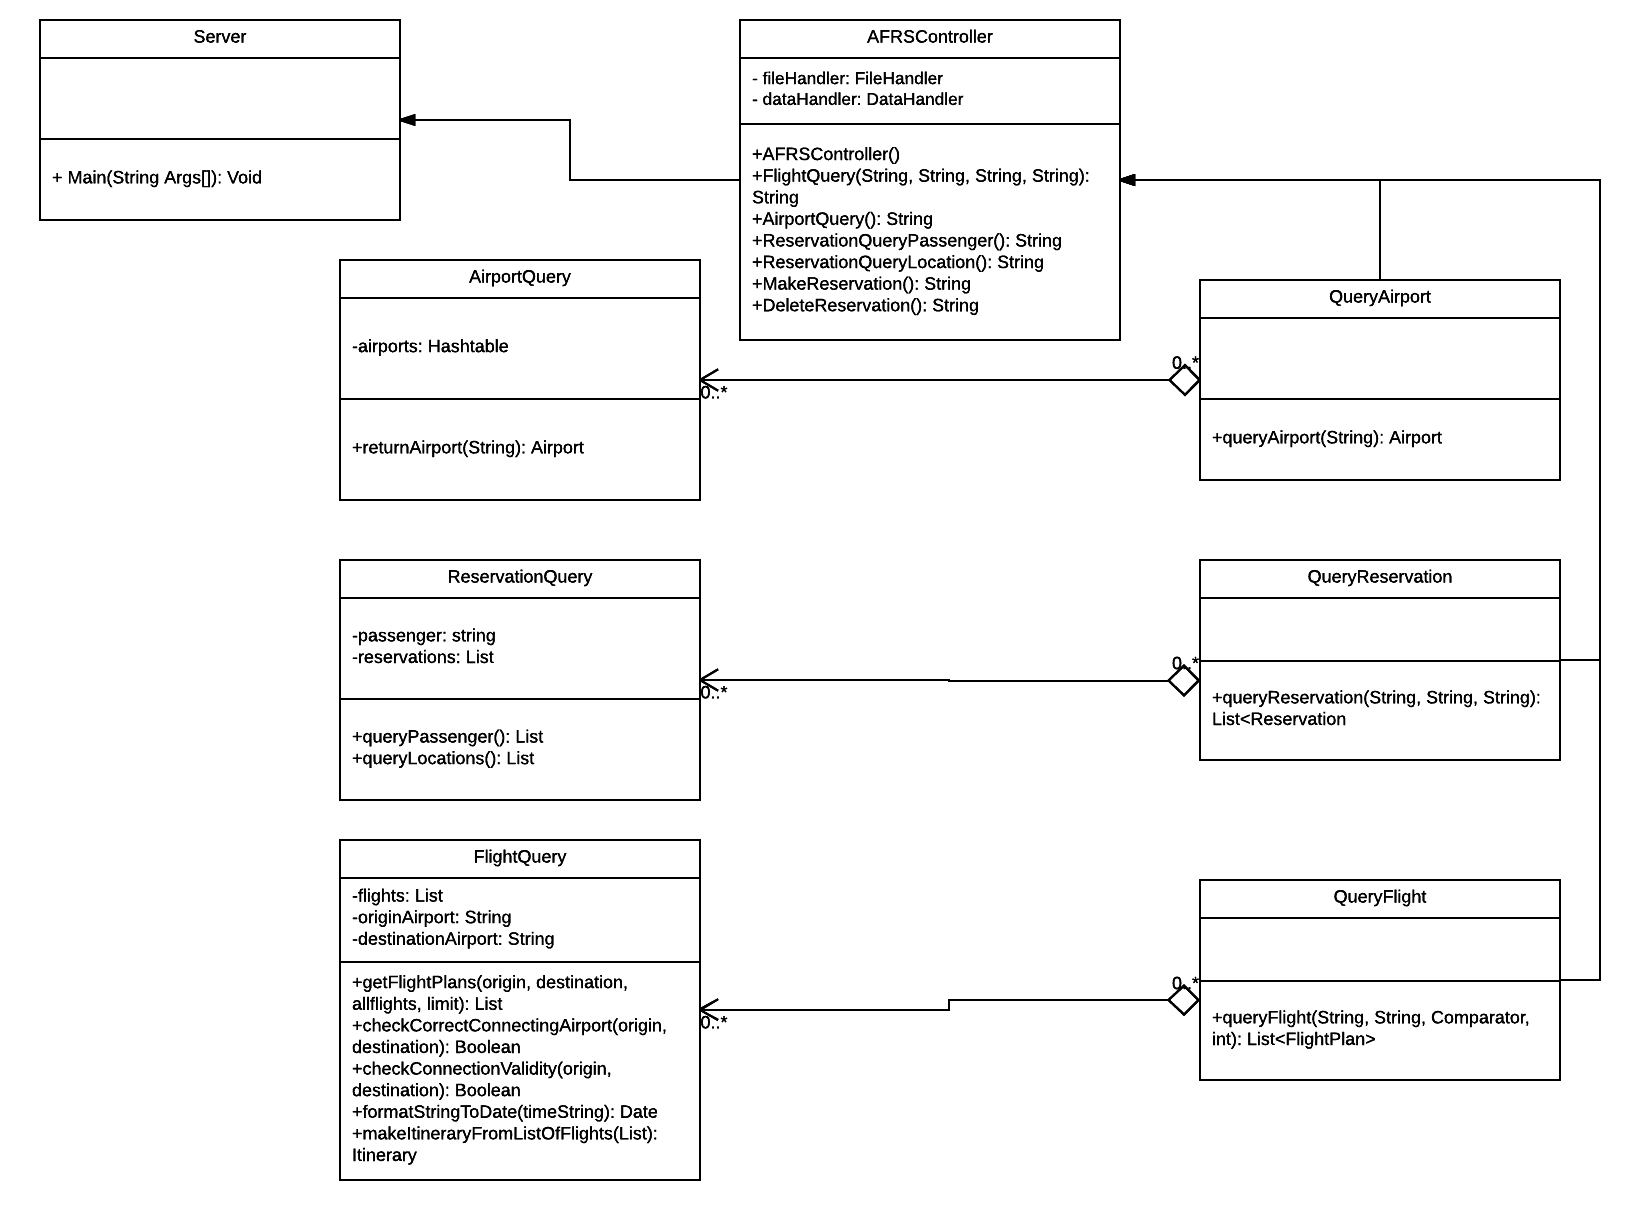
\includegraphics[width=\linewidth]{images/r2-proxy-class.png}}
\end{center}

\newpage

\subsubsection{Sequence Diagrams}

\paragraph{Release 2}

\begin{center}
    \makebox[\textwidth]{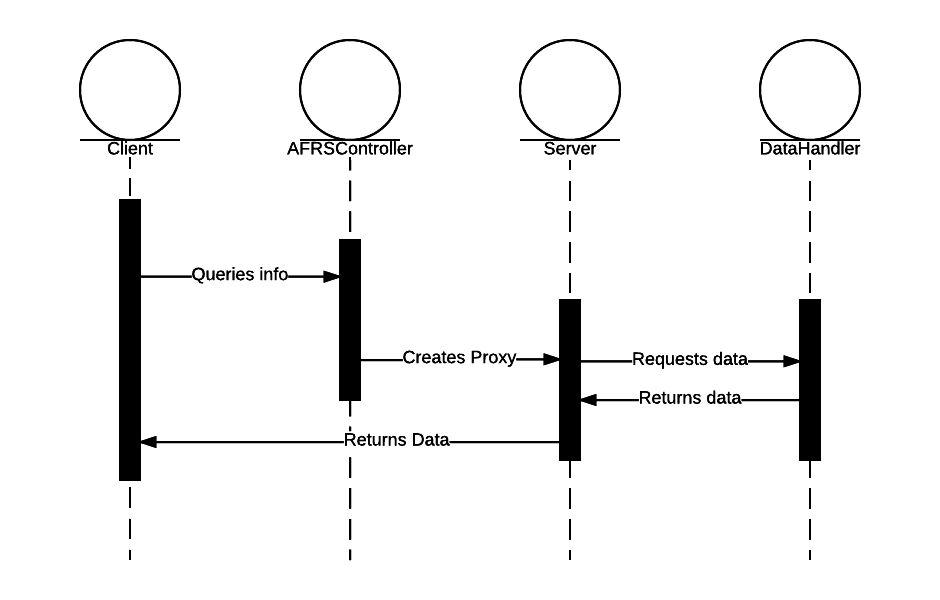
\includegraphics[width=\linewidth]{images/r2-proxy-sequence.png}}
\end{center}

\newpage

\subsubsection{GoF Card}

\begin{center}
    \begin{tabular}{ |p{4cm}|p{4cm}|p{7cm}|  }
        \hline
        \multicolumn{2}{|c|}{Name: Proxy} & \multicolumn{1}{|c|}{GoF pattern: Proxy} \\
        \hline
        \multicolumn{3}{|c|}{Participants} \\
        \hline
        Class & Role in GoF pattern & Participant's contribution in the context of the application \\
        \hline \hline

        CreateReservationProxy & Proxy & Makes a call to the Make Reservation Route on the server to create a reservation with the matching object information.\\
        \hline
        /MakeReservationQuery & Real Subject & Route for performing the actual reservation creation. This is done on the server regardless of which client made the request. Once it has made the request, all clients will be able to see this reservation in the system.\\
        \hline
        DeleteReservationProxy & Proxy & Makes a call to the Delete Reservation Route on the server to delete the reservation matching the object information sent over.\\
        \hline
        /DeleteReservationQuery & Real Subject & Route for performing the actual reservation deletion. This is done on the server regardless of which client made the request. Once it has deleted the reservation all clients will no longer be able to see the reservation in the system.\\
        \hline
        QueryAirport & Proxy &
        Makes a call to the Airport Query on the Server and returns the airport object that the server returns
        \\
        \hline
    \end{tabular}
    \begin{tabular}{ |p{4cm}|p{4cm}|p{7cm}|  }
        \hline
        Class & Role in GoF pattern & Participant's contribution in the context of the application \\
        \hline \hline
        /AirportQuery & Real Subject &
        Searches either the FAA or local files to return the airport object of the request, then returns it.
        \\
        \hline
        QueryFlight & Proxy &
        Makes a call to the Flight Query on the server and receives the flights and itineraries that exist on the server given the information provided.
        \\
        \hline
        /FlightQuery & Real Subject &
        Searches through its collection of flights and itineraries to return a list of FlightPlans to the client making the request.
        \\
        \hline
        QueryReservation & Proxy &
        Makes a call to the Query Reservation on the server and recieves Reservations given a passenger name.
        \\
        \hline
        /ReservationQueryPassenger & Real Subject &
        Searches through existing reservations for any reservations matching the queried passenger name and returns all matching objects to the client.
        \\
        \hline

        \hline
        \multicolumn{3}{|c|}{Deviations from the Pattern:} \\ \multicolumn{3}{|c|}{\parbox{0.9\textwidth}{
        \begin{itemize}
            \item Proxy and subject classes do not implement an interface.
        \end{itemize} }} \\
        \hline
        \multicolumn{3}{|c|}{Requirements being covered:} \\ \multicolumn{3}{|c|}{\parbox{0.9\textwidth}{
        \begin{itemize}
            \item The AFRS supports multiple clients but not truly concurrent clients.
        \end{itemize} }} \\
        \hline
    \end{tabular}
\end{center}

\newpage

%-------------------------------------------------------------------------------
% Subsystems / RESTFul Web Service
%-------------------------------------------------------------------------------
\subsection{RESTFul Web Service}\label{subsec:restfulWebService2}

One significant issue coming from release 1 was the coupling of our queries to the data handler.
With the introduction of a new multi-user requirement, we implemented a Facade Pattern, having our server controller (AFRSController) serve as the facade for all server subsystems to interact in one place.
What keeps it from being anti-pattern is how it is coupled;
none of the subsystems need to know about AFRSController, while direct coupling between queries and datahandler is kept minimal.

\subsubsection{Class Diagram}

\paragraph{Release 2}

\begin{center}
    \makebox[\textwidth]{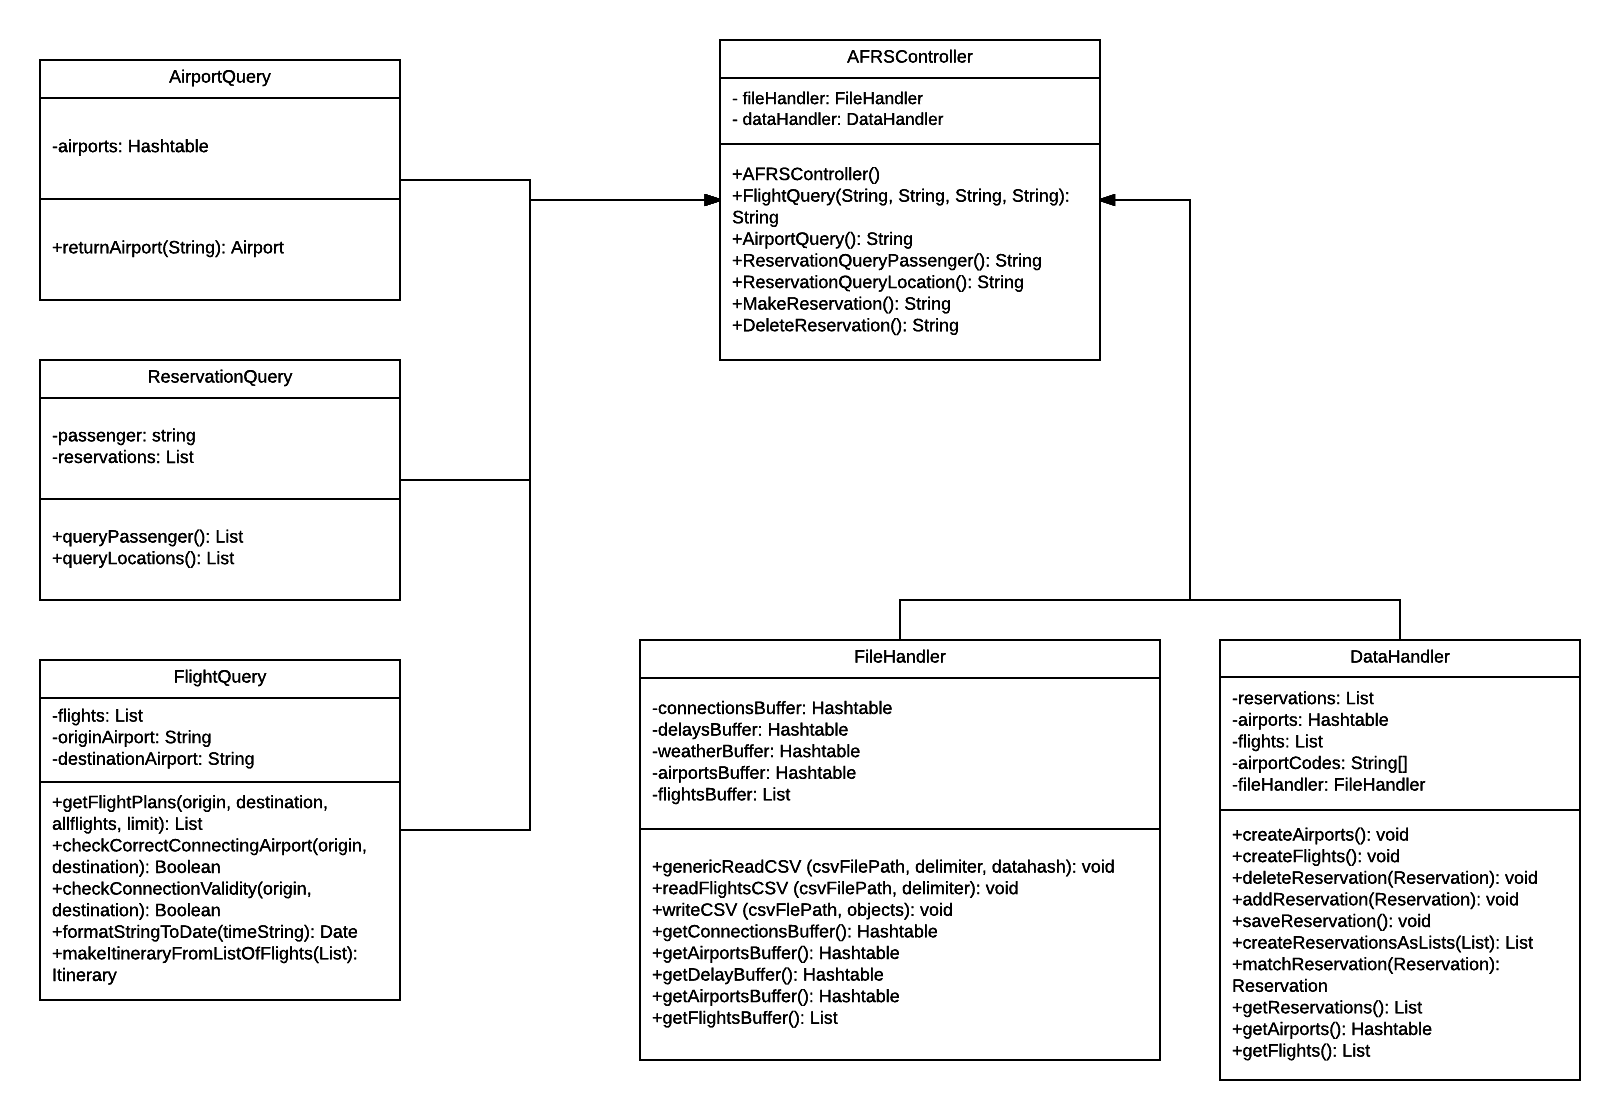
\includegraphics[width=\linewidth]{images/r2-AFRScontroller-class.png}}
\end{center}

\newpage

\subsubsection{Sequence Diagrams}

\paragraph{Release 2}

\begin{center}
    \makebox[\textwidth]{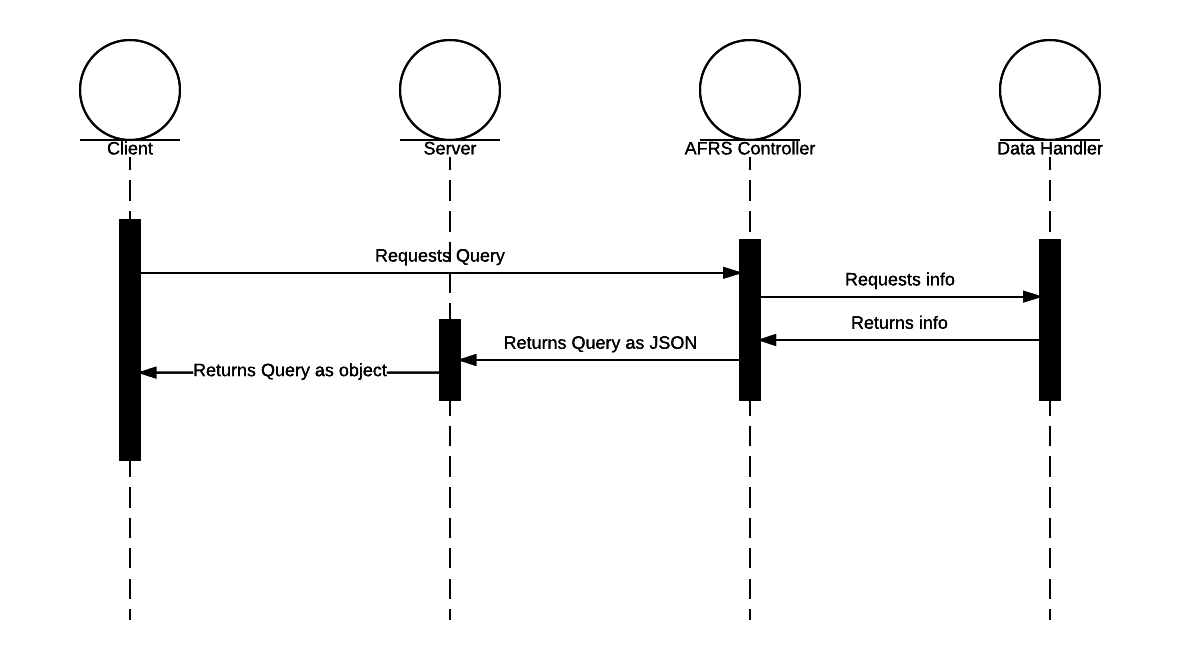
\includegraphics[width=\linewidth]{images/r2-AFRScontroller-sequence.png}}
\end{center}

\newpage

\subsubsection{GoF Card}

\begin{center}
    \begin{tabular}{ |p{4cm}|p{4cm}|p{7cm}|  }
        \hline
        \multicolumn{2}{|c|}{Name: RESTFul Web Service} & \multicolumn{1}{|c|}{GoF pattern: Facade} \\
        \hline
        \multicolumn{3}{|c|}{Participants} \\
        \hline
        Class & Role in GoF pattern & Participant's contribution in the context of the application \\
        \hline \hline

        AFRSController & Facade & Encapsulates all queries with datahandler and calls queries server-side using the datahandler. \\
        \hline
        AirportQuery & SubsystemA &
        Returns an airport object
        \\
        \hline
        ReservationQuery & SubsystemA &
        Returns a list of reservations by passenger name or origin and destination airports
        \\
        \hline
        FlightQuery & SubsystemA &
        Returns a list of flight plans
        \\
        \hline
        DataHandler & SubsystemB &
        Provides queried data from local or FAA
        \\
        \hline

        \hline
        \multicolumn{3}{|c|}{Deviations from the Pattern:} \\ \multicolumn{3}{|c|}{\parbox{0.9\textwidth}{
        \begin{itemize}
            \item SubsystemB’s DataHandler is instantiated in the SubsystemA classes directly for construction.
            \item Facade does add some new functionality related to server interaction
            \item Facade is not an interface
        \end{itemize} }} \\
        \hline
        \multicolumn{3}{|c|}{Requirements being covered:} \\ \multicolumn{3}{|c|}{\parbox{0.9\textwidth}{
        \begin{itemize}
            \item Server and client interactions enabling multi-concurrent users.
        \end{itemize} }} \\
        \hline
    \end{tabular}
\end{center}

\newpage

%-------------------------------------------------------------------------------
% Subsystems / FAA or Local State
%-------------------------------------------------------------------------------
\subsection{FAA or Local State}\label{subsec:faaOrLocalState}

\indent
One new requirement in R2 was to allow the user to fetch information from FAA services instead of local. The system initially loads from local anyway, which we believed made it a good fit for the State Pattern. It has an obvious default state (local) and can transition to FAA on request and back. Additionally it only loads local by default, which makes the system load faster than having to load both simultaneously (in case the user never wishes to fetch from FAA). This also makes state transitions after the first one faster since local and FAA remain loaded.

\subsubsection{Class Diagram}

\paragraph{Release 2}

\begin{center}
    \makebox[\textwidth]{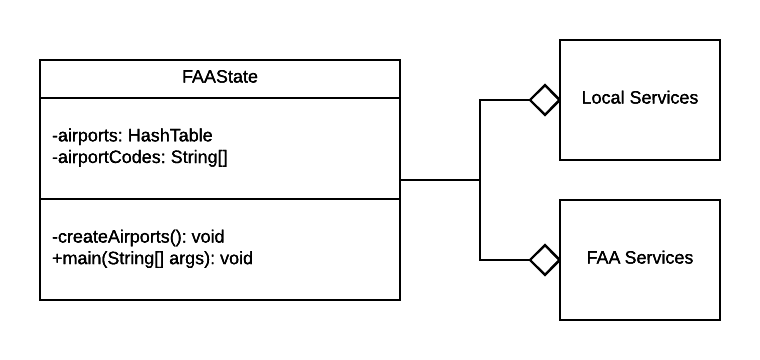
\includegraphics[width=\linewidth]{images/R2-FAA-State.png}}
\end{center}

\subsubsection{State Diagram}

\paragraph{Release 2}

\begin{center}
    \makebox[\textwidth]{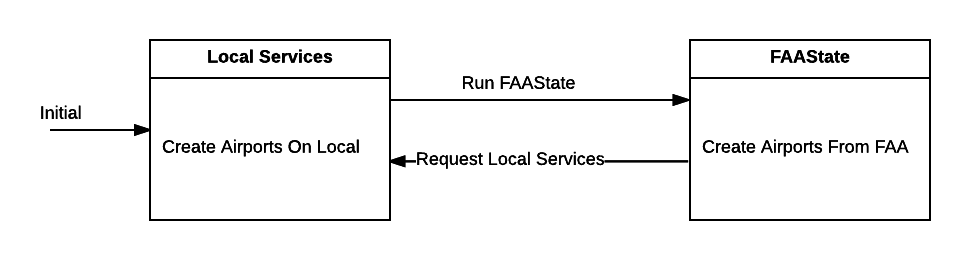
\includegraphics[width=\linewidth]{images/r2-FAA-state.png}}
\end{center}

\subsubsection{Sequence Diagrams}

\paragraph{Release 2}

\begin{center}
    \makebox[\textwidth]{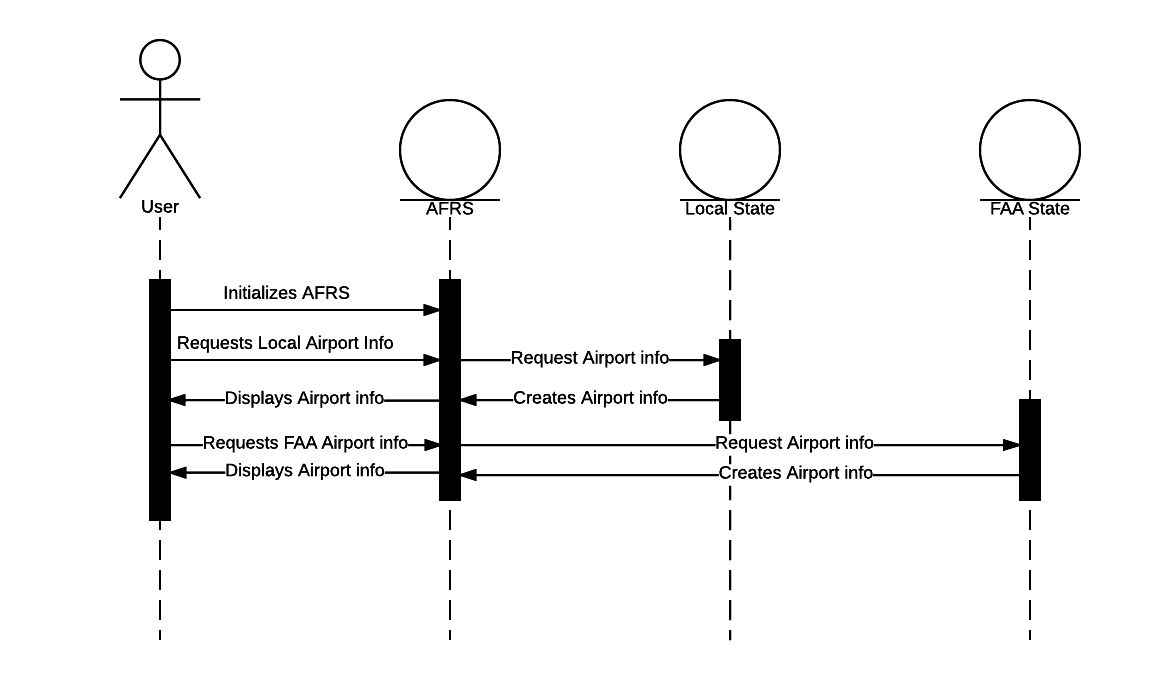
\includegraphics[width=\linewidth]{images/r2-FAA-sequence.png}}
\end{center}

\subsubsection{GoF Card}

\begin{center}
    \begin{tabular}{ |p{4cm}|p{4cm}|p{7cm}|  }
        \hline
        \multicolumn{2}{|c|}{Name: FAA or Local State} & \multicolumn{1}{|c|}{GoF pattern: State} \\
        \hline
        \multicolumn{3}{|c|}{Participants} \\
        \hline
        Class & Role in GoF pattern & Participant's contribution in the context of the application \\
        \hline \hline

        FAAState & ConcreteState &
        Enables system to read data from FAA service only if the client requests it.
        \\
        \hline

        \hline
        \multicolumn{3}{|c|}{Deviations from the Pattern:} \\ \multicolumn{3}{|c|}{\parbox{0.9\textwidth}{
        \begin{itemize}
            \item State does not implement an interface
        \end{itemize} }} \\
        \hline
        \multicolumn{3}{|c|}{Requirements being covered:} \\ \multicolumn{3}{|c|}{\parbox{0.9\textwidth}{
        \begin{itemize}
            \item Provides the user the ability to view airport information either from local services or FAA.
        \end{itemize} }} \\
        \hline
    \end{tabular}
\end{center}

\newpage
    